%
% komplex.tex
%
% (c) 2018 Prof Dr Andreas Müller, Hochschule Rapperswil
%
\subsubsection{Komplexe Fouriertransformation}
Bisher wurden alle Rechnungen nur mit reellen Zahlen durchgeführt.
Es stellt sich aber heraus, dass komplexe Zahlen für die Beschreibung
der Fourier-Transformation sehr viel praktischer sind.
Der Grund dafür ist die Eulersche Beziehung
\[
e^{it} = \cos t + i \sin t
\]
und die Rechenregel
\[
e^{a+b}=e^a\cdot e^b
\qquad\Rightarrow\qquad
e^{ikt}=\cos kt+i\sin kt = (\cos t + i \sin t)^k
\]
für die Exponentialfunktion.
Im Folgenden gehen wir wieder von $N=2n$ aus.

Die reellen Fourier-Koeffizienten werden durch die Summen
\[
a_0
=
\frac{1}{N}\sum_{j=1}^N y_j,\quad
a_l
=
\frac{2}{N}\sum_{j=1}^N y_j \cos lt_j
\quad\text{und}\quad
b_l
=
\frac{2}{N}\sum_{j=1}^N y_j \sin lt_j
\]
berechnet.
Für $l=0$ liefert die Formel für $b_l$ trivialerweise $b_0=0$.
Für $l=n$ ist $\sin lt_j = \sin nt_j = \sin \pi j=0$, also verschwindet auch
die Summe für $b_n$.
Fassen wir $a_l$ und $b_l$ als Real- und Imaginärteil einer komplexen
Zahl auf, dann können wir 
\begin{align}
c_0
&=
a_0-ib_0
=
\frac{1}{N}
\sum_{j=1}^N y_j
=
\frac{1}{N}
\sum_{j=1} y_j e^{-0t_j}
\label{skript:complex:c0}
\\
c_l
&=
\frac12(a_l-ib_l)
=
\frac{1}{N} \sum_{j=1}^N y_j (\cos lt_j - i \sin lt_j)
=
\frac1{N} \sum_{j=1}^N y_j e^{-lt_j}
%=
%\frac{1}{N} \sum_{j=1}^N y_j e^{-2\pi ilj/N}
\label{skript:complex:cl}
\\
c_n
&=
\frac12(a_n-ib_n)
=
\frac{1}{N} \sum_{j=1}^N y_j (\cos nt_j  -i\sin nt_j)
=
\frac{1}{N} \sum_{j=1}^N y_j e^{-int_j}
=
\frac{1}{N} \sum_{j=1}^N y_j (-1)^j
\label{skript:complex:cn}
\end{align}
berechnen.

Für reelle Werte $y_j$ haben die Koeffizienten $c_l$ zusätzliche
Symmetrieeigenschaften.
Die komplex konjugierten Koeffizienten $\bar c_l$ ist
\[
\bar c_l
=
\overline{\sum_{j=0}^{N-1} y_j e^{-ilt_j}}
=
\sum_{j=0}^{N-1} y_j e^{ilt_j}
=
c_{-l}.
\]
Ausserdem ist $c_{N-l}=c_{-l}$ wegen $e^{\pm iNt_j}=1$.
Zusammen mit der Beziehung $\bar c_l=c_{-l}$, können wir die komplexen
Fourier-Koeffizienten auch verwenden, um die reellen Koeffizienten
\begin{equation}
\begin{aligned}
a_l
&=
c_l + c_{-l}
&&\text{und}&
ib_l
&=
-c_l + c_{-l}
\end{aligned}
\end{equation}
durch die komplexen Koeffizienten auszudrücken.

Auch die Rekonstruktion~\eqref{skript:fourier:rekonstruktion} ist
mit komplexen Zahlen darstellbar.
Dazu verwendet man 
\[
\cos x = \operatorname{Re} e^{ix} = \frac{e^{ix}+e^{-ix}}{2}
\qquad\text{und}\qquad
\sin x = \operatorname{Im} e^{ix} = \frac{e^{ix}-e^{-ix}}{2i}.
\]
Damit wird das trigonometrische Polynom
\begin{align*}
f(t_j)
&=
a_0
+\sum_{k=1}^{n-1} (a_k \cos kt_j + b_k \sin kt_j)
+a_n \cos nt_j
\\
&=
a_0
+\sum_{k=1}^{n-1} (a_k \operatorname{Re} e^{ikt_j} + b_k\operatorname{Im}e^{ikt_j})
+ a_n e^{int_j}
\\
&=
c_0
+
\sum_{k=0}^{n}
\frac12
\bigl(
(a_k-ib_k) e^{ikt_j}
+
(a_k+ib_k) e^{-ikt_j}
\bigr)
+
c_n e^{int_j}
\\
&=
c_0
+
\sum_{k=0}^{n}
\biggl(
\frac12
(a_k-ib_k) e^{ikt_j}
+
\frac12
(a_k+ib_k) e^{-ikt_j}
\biggr)
+
c_n e^{int_j}.
\intertext{Zusammen mit den Koeffizienten $c_{-l}$ folgt}
&=
c_0
+
\sum_{k=0}^{n-1} \bigl(c_k e^{ikt_j} + \bar{c}_k e^{-ikt_j})
+
c_n e^{int_j}
\\
&=
c_0
+
\sum_{k=1}^{n-1}(c_ke^{ikt_j} + c_{-k}e^{-ikt_j})
+
c_n e^{int_j}
=
\sum_{k=-n+1}^n c_k e^{ikt_j}
=
\sum_{k=0}^{N-1} c_k e^{ikt_j}.
\end{align*}
Damit sieht die Rekonstruktionsformel bis auf das Vorzeichen
im Exponenten gleich aus wie die
Transformationsformel~\eqref{skript:complex:cl}.
Diese Eigenschaft kann dazu verwendet werden, die Rücktransformation
im Wesentlichen mit demselben Code zu berechnen wie die Transformation.
Wir fassen die Resultate im folgenden Satz zusammen.

\begin{satz}
Sei $N=2n$ und $t_j=2\pi j/N$, und seien Funktionswerte $y_j\in\mathbb C$
geben.
Dann ist
\[
c_l = \sum_{j=1}^N y_j e^{-ilt_j}
\qquad
\Rightarrow
\qquad
y_j = \sum_{k=0}^{N-1} c_ke^{ikt_j}.
\]
Falls $y_j\in\mathbb R$, dann ist $c_{-l}=c_l$, $c_0,c_n\in\mathbb R$.
\end{satz}

\subsubsection{Spektrum}
\begin{figure}
\centering
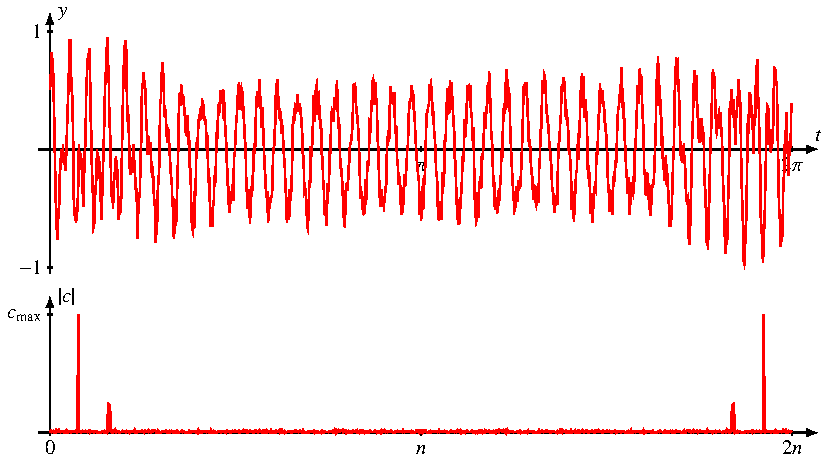
\includegraphics{chapters/6/spektrum.pdf}
\caption{Graphische Darstellung von Funktion und Spektrum
\label{skript:komplex:spektrum}}
\end{figure}
Die Koeffizienten $c_k$ zeigen an, mit welcher Amplitude die Schwingung
$e^{ikt}$ in der Funktion $f(t)$ vertreten ist.
In Abbildung~\ref{skript:komplex:spektrum} ist oben die Funktion 
\[
f(t)
=
0.5 \cos 40t
+0.1\sin 80t
+0.12\sin 81t
+0.12\sin 82t
+0.1\sin 83t
+g(t)
\]
dargestellt, wobei $g(t)$ ein zufälliges Rauschsignal ist.
In der unteren Graphik sind die Beträge $|c_k|$ der Koeffizienten $c_k$ 
dargestellt.
Die Skala ist so gewählt, dass
\[
c_{\text{max}} = \max_{1\le k\le N} |c_k|.
\]
Man nennt $c_k$ auch das {\em Spektrum} von $f$.
\index{Spektrum}%

